\documentclass[12pt,a4paper,oneside]{ctexart}
\usepackage{caption,graphicx,amsmath,amsthm,amsfonts,amssymb,bm,mathrsfs,extarrows,
indentfirst,setspace,textcomp,xcolor,color,colortbl,booktabs,float,subcaption,
fancyhdr}
\usepackage[centering]{geometry}
\usepackage{array,blkarray}
\usepackage{tikz,tikz-3dplot,asymptote}
\usepackage{listings}

\geometry{left=2.54cm,right=2.54cm,top=3.18cm,bottom=3.18cm}
\usetikzlibrary{arrows.meta}
\setlength{\headheight}{15pt}
\newfontfamily\consolas{Consolas}
\definecolor{lightgray}{gray}{0.5}
\linespread{1.5}

\newcommand{\dif}{\mathrm{d}}
\newcommand{\differ}{\backslash}
\newcommand{\ptl}{\partial}
\newcommand{\R}{\mathbb{R}}
\newcommand{\N}{\mathbb{N}}
\newcommand{\C}{\mathbb{C}}
\newcommand{\D}{\mathbb{D}}
\newcommand{\Z}{\mathbb{Z}}
\renewcommand{\phi}{\varphi}
\renewcommand{\epsilon}{\varepsilon}
\newcommand{\abs}[1]{\left\vert#1\right\vert}
\newcommand{\norm}[1]{\left\Vert#1\right\Vert}

\title{思路}
\date{}
\author{}

\begin{document}

  \maketitle

\subsection*{第一问}

假设:
\begin{enumerate}
  \item 每辆货车完全相同.
  \item 忽略货车长度.
  \item 货车在$P$点和$D$点不耗电.
  \item 货车匀速行驶,忽略启动和停止的所需的时间.
  \item 在换电站不装卸货.
  \item 更换电池时6个电池同时更换.
  \item 在换电站更换车辆不需要耗费时间.
  \item ……
\end{enumerate}

设换电站为$Q$,它到$P$的距离是$s$km,货车以60km/h在路上行驶的时间与$s$无关,都是$\frac{1}{3}$h.设在公路上行驶的货车共$n$辆,因为车距至少$0.2$km,那么
\begin{equation}
  0.2n\leqslant 20.
\end{equation}
为了极大化运货量,这些货车都应该当前一辆车启动之后第一次与换电站距离至少0.2km出发.按照最开始启动的顺序从1到$n$编号,接下来假设在1000h中,1号货车行驶过程中换电次数是$N$次.令$k\leqslant N$,$x_i(k)$表示第$i$辆车在第$k-1$次换电之后,$k$次换电之前与前车的间距,$1\leqslant i\leqslant n$,对第1辆车来说是与第$n$辆车的 
间距,令$x_{n+1}(k)=x_1(k)$,$x_{i}(N+1)$表示在第$N$次换电后$i$车与前车的间距.记$i$车第$k-1$次换电之后,$k$次换电之前行驶的圈数是$a_i(k)$,$a_i(N+1)$表示在第$N$次换电后行驶的圈数,规定$a_i(0)=0$,这里允许$a_i(k)$是小数,小数部分$\{a_i(k)\}$表示在行进$[a_i(k)]$圈之后又行驶了$20\{a_i(k)\}$km.
那么可以得到
\begin{gather}
  x_i(k)\geqslant 0.2,i=1\cdots,n,k=1,\cdots,N+1.\\
  x_1(k)+\cdots+x_n(k)=20,k=1,\cdots,N+1.
\end{gather}
而且,因为$n$车行驶到1车的位置所需时间最多不超过$\frac{1}{3}+\frac{1}{30}=\frac{11}{30}$h,小于电池充好电的时间3h,所以,剩余没有使用的电池(包括备用
的车的电池)要不少于车中的电池,
\begin{equation}
  900-60n\cdot 2\geqslant 0.
\end{equation}

{\color{red}那么$N\leqslant 75$,为了极大化运货量,令$N=75$.}

另外,货车每次换电有几种选择:1.当空载时,可以选择更换车辆,也可以选择更换电池;2.当载着货物时,只能选择更换电池.所以用$m(k)$表示所有在第$k$次换电时更换车辆的数目,$n-m(k)$表示所以
在第$k$次换电时更换电池的车辆数.$m(k)$必须小于在换电站备用的货车数,满足
\begin{equation}
  m(k)\leqslant 125-n,k=1,2,\cdots,N.
\end{equation}
同样,剩余的电池数不少于需要更换的电池数,
\begin{equation}
  6(n-m(k))\leqslant 150.
\end{equation}

\begin{figure}[H]
  \centering
  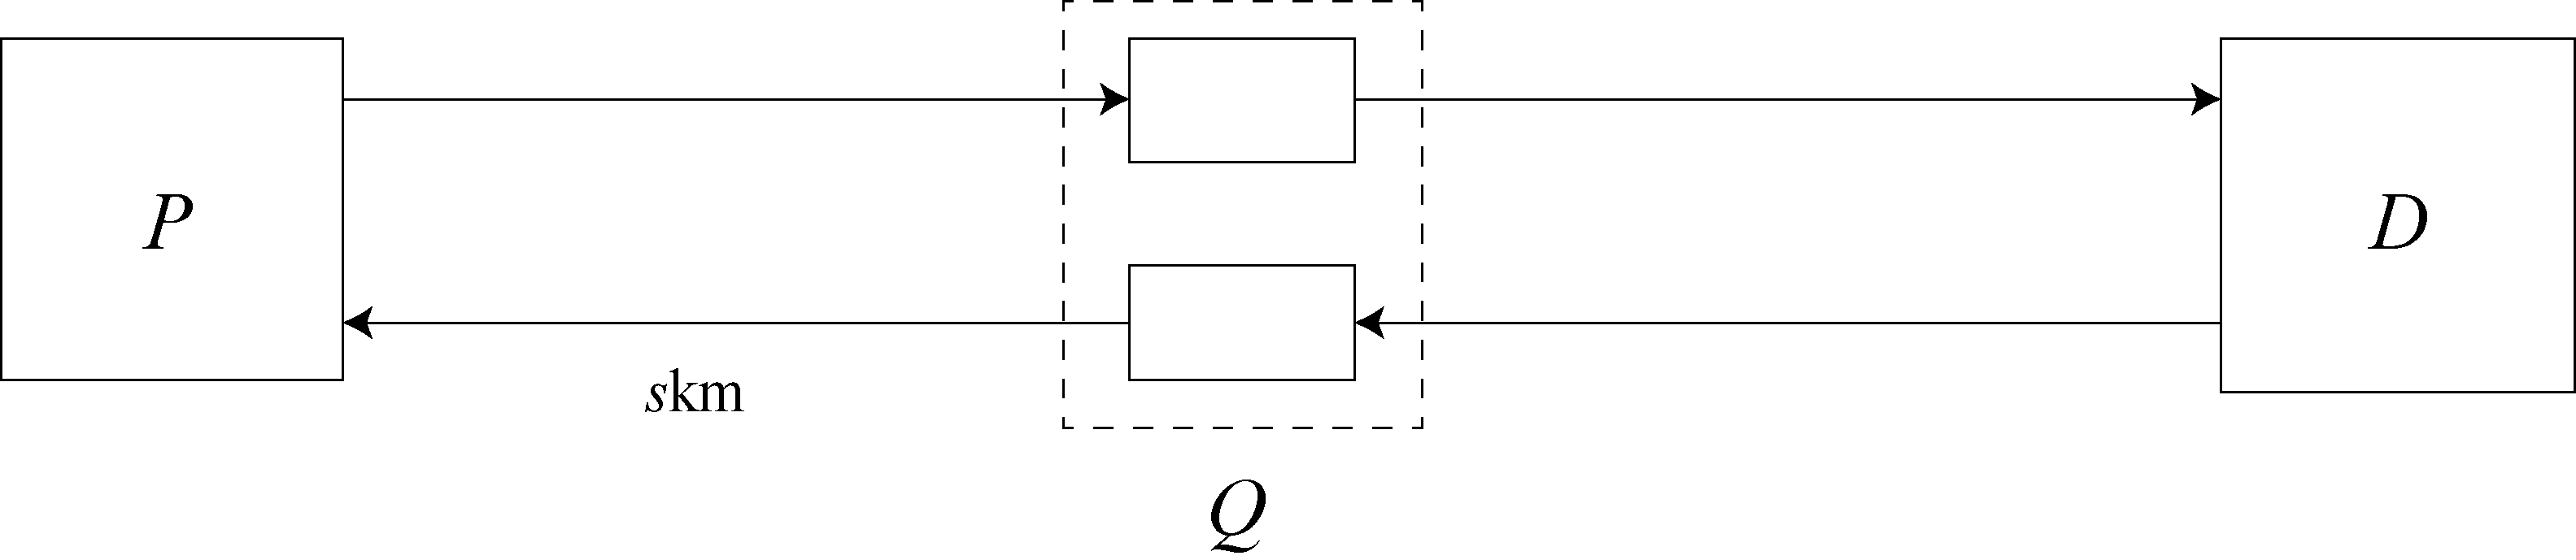
\includegraphics[scale=0.25]{资源 1.pdf}
  \caption{第一问示意图}
\end{figure}

对每个$k$,$j$从1到$n$遍历,当$j$车换电时,要求电量在$[10\%,25\%]$,$a_j(k)$表示$j$车第$k-1$次换电之后,$k$次换电之前走的圈数,
\begin{gather}
  10\leqslant 100-\frac{25}{3}a_j(k)\leqslant 25,k=1,\cdots,N.\\
  10\leqslant 100-\frac{25}{3}a_j(N+1).
\end{gather}
而且$\{a_j(k)\}\ (k=1,\cdots,N)$取值可以确定,当$\{a_j(0)+\cdots+a_j(k-1)\}=0$时,$\{a_j(k)\}=\frac{s}{10}$或0,当$\{a_j(0)+\cdots+a_j(k-1)\}\neq 0$时,$\{a_j(k)\}=\frac{10-s}{10}$或0.

这时,$j$货车位置有两种情况:1.在从$D$到$P$方向的换电站,此时货车空载,累计圈数是整数,
\begin{equation}
  \{a_j(1)+\cdots+a_j(k)\}=0.
\end{equation}
这时可以选择换车还是换电池.2.在从$P$到$D$方向的换电站,这时货车载着货物,累计圈数不是整数,
\begin{equation}
  \{a_j(1)+\cdots+a_j(k)\}>0.
\end{equation}
这时只能换电池.接下来引入变量$y_i(k)$,表示$i$车前车在第$k$次换电后与$i$车的车距.令$y_1(k)=x_1(k),y_{n+1}(k)=y_1(k)$.

对于第一种情况,因为换车不消耗时间,换电池消耗时间,所以不同的操作可能会改变前后车的间距.当$y_j(k)\geqslant 0.2$,可以换车,这时车距变化是:
\begin{gather}
  x_j(k+1)=y_j(k),\\
  y_{j+1}(k)=x_{j+1}(k).
\end{gather}
如果换电池的话,
\begin{gather}
  x_j(k+1)=y_j(k)+2,\label{eq:换电池x_j}\\
  y_{j+1}(k)=x_{j+1}(k)-2.\label{eq:换电池y_j+1}
\end{gather}
当$y_j(k)<0.2$,只能换电池,\eqref{eq:换电池x_j}和\eqref{eq:换电池y_j+1}成立.

对于第二种情况,只能换电池,同样\eqref{eq:换电池x_j}和\eqref{eq:换电池y_j+1}成立.

然后,因为$k$次换电时候换车最多$m(k)$辆,用$c_i(k)$表示$i$车第$k$次换电是否换电池,令
\begin{equation}
  c_i(k)=\begin{cases}
    0 & \mbox{不换电池},\\
    1 & \mbox{换电池}.
  \end{cases}
\end{equation}
和$d_i(k)=1-c_i(k)$,那么
\begin{equation}
  d_1(k)+\cdots+d_n(k)=m(k).
\end{equation}

接下来设$i\ (i=1,\cdots,N+1)$车第$k-1$次换电后,第$k$次换电前到达$D$的次数是$z_i(k)$,其实就是运货量,那么它和$a_i(k)$有以下关系:
\begin{equation}
  z_i(k)=\begin{cases}
    [a_i(k)]+1 & \{a_i(k)\}\geqslant \frac{10+s}{20},\\
    [a_i(k)] & \{a_i(k)\}<\frac{10+s}{20}.
  \end{cases}
\end{equation}
那么极大化的目标函数是
\begin{equation}
  \sum_{i=1}^n\sum_{j=1}^Nz_i(j).
\end{equation}

记1车第$k-1$次换电后,$k$次换电前用时是$t(k)$,$t(N+1)$表示第$N$次之后运行时间.包括:1.在公路上行驶的用时,共$\frac{a_1(k)}{3}$h.2.装卸货用时,当$0\leqslant \{a_1(k)\}\leqslant \frac{s}{20}$或
$\frac{10+s}{20}\leqslant \{a_1(k)\}<1$时,共用时$\frac{z_1(k)}{30}$h,当$\frac{s}{20}\leqslant \{a_1(k)\}<\frac{10+s}{20}$时,用时$\frac{z_(k)}{30}+\frac{1}{60}$h.
所以 
\begin{equation}
  t(k)=\frac{a_1(k)}{3}+\begin{cases}
    \frac{z_1(k)}{30} & 0\leqslant \{a_1(k)\}\leqslant \frac{s}{20}\mbox{或}\frac{10+s}{20}\leqslant \{a_1(k)\}<1,\\
    \frac{z_1(k)}{30}+\frac{1}{60} & \frac{s}{20}\leqslant \{a_1(k)\}<\frac{10+s}{20}.
  \end{cases}
\end{equation}
换电池总时间$\frac{1}{30}\sum_{j=1}^Nc_1(j)$,那么
\begin{equation}
  t(1)+\cdots+t(N+1)+\frac{\sum_{j=1}^Nc_1(j)}{30}\leqslant 1000.
\end{equation}

\end{document}





用货车运货次数,也就是到达$D$点次数来衡量运货量.设在公路上共有$N$辆车,每辆车间距不少于200m,得到不等式
\begin{equation}
  \label{eq:N的简单估计}
  \frac{20}{N}\geqslant 0.2.
\end{equation}
得到$N\leqslant 100$.同时,对公路上的车从开始依次标号,记为1,2,$\cdots$,$N$,为了尽量最大化货物量,当货车与换电站隔200m时就发出下一辆车.从第1辆车换电结束到第$N$辆车换电时间间隔不超过$20/60=1/3$h,也就是说从第1辆货车换电结束到
第$N$辆车换电开始没有换下来的电池能进入备用状态.另外,因为$N\leqslant 100<125$,也就是说此时还有车没有出发,所以在换电站有不同种选择:1.当货车空载换电时,可以选择直接更换车辆
或者更换电池,前者不需要耗费时间,后者要耗费$20\times 6=120$s时间;2.当货车载着货物换电时,只能换电池,同样耗费120s时间.

因为从第1辆货车换电结束到第$N$辆车换电开始没有换下来的电池能进入备用状态,所以需要考虑去掉这$N$辆车的电池剩下的电池(包括剩下车里面的电池)是否够用,那么得到
\begin{equation}
  \label{eq:N的精确估计}
  900-6N-6N\geqslant 0.
\end{equation}
结合式\eqref{eq:N的简单估计}和\eqref{eq:N的精确估计},得到$N\leqslant 75$.因为车速确定,所以第1辆车往返一次运输的总货物和$N$正相关,要想1000h运送货物量最大,取$N=75$,此时使用的电池数量
恰好等于剩余未使用的电池数量.

接下来考虑,换下来的电池能否在下一次充电的时候准备完毕.在每一圈中,设换电站$Q$到$P$点距离是$s$km,那么有4个过程:1.从$Q$到$P$是空载,用时$\frac{s}{60}$h,耗电$\frac{s}{3}\%$;
2.从$P$到$Q$是载着货物,时间也是$\frac{s}{60}$h,耗电$\frac{s}{2}\%$;3.从$Q$到$D$是载着货物,时间$\frac{10-s}{60}$h,耗电$\frac{10-s}{2}\%$;4.从$D$到$Q$是空载,时间$\frac{10-s}{60}$h,
耗电$\frac{10-s}{3}\%$.总共耗电$\frac{25}{3}\%$,这个与换电站的位置无关.换下来的电池需要3小时才能够使用,这段时间每辆车最多走$60\times 3=180$km,也就是9圈,耗电最多$75\%$,剩下的电量没有低于$10\%$,
所以这时能够使用换下来的电池.

在换电站可以进行3种操作:1.载着货物时只换电池;2.空载时可以换电池;3.空载时可以换车.如果存在换车的情况,假设有$k$辆车换车,其他公路上的车辆换电池,那么$k$不超过剩余的车辆数,也就是
\begin{equation}
  \label{eq:k的上界}
  k\leqslant 125-N=50.
\end{equation}
同时,剩下的$N-k$辆车用的电池数不超过剩余的电池数,
\begin{equation}
  \label{eq:k的下界}
  6(N-k)\leqslant 900-125\times 6=150.
\end{equation}
结合式\eqref{eq:k的上界}和\eqref{eq:k的下界},得到$k=50$.那么此时只能有$50$辆车换车,其实也说明这时候每次换电时,一定会有50辆车是空载换车,其他25辆车是换电池的.接下来
考虑到空载换车时不需要消耗时间,这样会缩小换车的车辆与前面换电池车辆的距离,缩短的距离是$20\times 6/3600\times 60=2$km.一辆从$100\%$SoC启动的货车在第9圈剩余电量$25\%$,在第10圈剩余电量$\frac{50}{3}\%$,
为了减少不必要的停留时间,采取以下措施:在第一次电量剩余$\frac{50}{3}\%$前,第1辆车与第75辆车间距5km,当第一次电量剩余$\frac{50}{3}\%$时,这时候空载,1-50号车换车,51-75号车换电池,此时第1辆车和第75辆车间隔3km,第二次电量剩余
$\frac{50}{3}\%$时,这时候仍然空载,令1-25,51-75号车换车,26-50号车换电池,此时第1辆车和第75辆车间距3km,第三次电量$\frac{50}{3}\%$时,这时候仍然空载,1-25号车换电池,26-75号车换车,此时车距全部恢复,之后循环往复.
